% ================================================================
%  LIGHT AS CAUSAL COHERENCE STRUCTURE
%  IN COMPACT S³ GEOMETRY
%
%  HCC Research Branch: Null Relational Propagation
%  and Compact Causal Accessibility
%
%  Andrei Preece & Boris Batenin
%  Berlin, 2026
% ================================================================
\documentclass[12pt,a4paper]{article}

\usepackage[T1]{fontenc}
\usepackage[utf8]{inputenc}
\usepackage{microtype}
\microtypesetup{expansion=false}
\usepackage{geometry}
\geometry{a4paper,top=2.5cm,bottom=2.5cm,left=2.8cm,right=2.8cm}

%% --- Math ---
\usepackage{amsmath,amssymb,amsthm,mathtools}
\usepackage{mathrsfs}
\usepackage{bm}

%% --- TikZ / Figures ---
\usepackage{tikz}
\usepackage{pgfplots}
\pgfplotsset{compat=1.17}
\usetikzlibrary{calc,decorations.pathmorphing,arrows.meta,
  patterns,positioning,shapes.geometric,3d}

%% --- Layout ---
\usepackage{setspace}
\setstretch{1.17}
\usepackage{parskip}
\setlength{\parskip}{5pt plus 1pt}
\setlength{\parindent}{0pt}
\usepackage{enumitem}
\usepackage{caption}
\captionsetup{font=small,labelfont=bf}

%% --- Tables ---
\usepackage{booktabs,tabularx,array}
\usepackage[table,dvipsnames]{xcolor}

%% --- Colors ---
\definecolor{hdrblue}{RGB}{15,70,130}
\definecolor{thmgreen}{RGB}{224,244,224}
\definecolor{thmframe}{RGB}{25,112,38}
\definecolor{defblue}{RGB}{222,237,252}
\definecolor{defframe}{RGB}{15,70,130}
\definecolor{propvio}{RGB}{243,233,252}
\definecolor{propframe}{RGB}{90,32,142}
\definecolor{conjcol}{RGB}{255,248,220}
\definecolor{conjframe}{RGB}{150,110,5}
\definecolor{philocol}{RGB}{238,252,246}
\definecolor{philoframe}{RGB}{18,125,95}
\definecolor{alertcol}{RGB}{252,232,230}
\definecolor{alertframe}{RGB}{150,35,15}
\definecolor{limcol}{RGB}{245,245,245}
\definecolor{limframe}{RGB}{118,118,118}
\definecolor{remarkbg}{RGB}{249,249,249}
\definecolor{remarkfr}{RGB}{135,135,135}
\definecolor{rowA}{RGB}{232,242,252}
\definecolor{rowB}{RGB}{251,251,253}

%% --- Coloured boxes ---
\usepackage{tcolorbox}
\tcbuselibrary{most}
\tcbset{
  thmbox/.style={colback=thmgreen,colframe=thmframe,
    fonttitle=\bfseries,title={#1},
    left=7pt,right=7pt,top=5pt,bottom=5pt,
    sharp corners,boxrule=1pt,parbox=false},
  defbox/.style={colback=defblue,colframe=defframe,
    fonttitle=\bfseries,title={#1},
    left=7pt,right=7pt,top=5pt,bottom=5pt,
    sharp corners,boxrule=1pt,parbox=false},
  propbox/.style={colback=propvio,colframe=propframe,
    fonttitle=\bfseries,title={#1},
    left=7pt,right=7pt,top=5pt,bottom=5pt,
    sharp corners,boxrule=1pt,parbox=false},
  conjbox/.style={colback=conjcol,colframe=conjframe,
    fonttitle=\bfseries\itshape,title={#1},
    left=7pt,right=7pt,top=5pt,bottom=5pt,
    sharp corners,boxrule=0.9pt,parbox=false},
  philobox/.style={colback=philocol,colframe=philoframe,
    fonttitle=\bfseries\itshape,title={#1},
    left=7pt,right=7pt,top=5pt,bottom=5pt,
    sharp corners,boxrule=0.8pt,parbox=false},
  alertbox/.style={colback=alertcol,colframe=alertframe,
    fonttitle=\bfseries,title={#1},
    left=7pt,right=7pt,top=5pt,bottom=5pt,
    sharp corners,boxrule=1pt,parbox=false},
  limbox/.style={colback=limcol,colframe=limframe,
    fonttitle=\bfseries\itshape,title={#1},
    left=7pt,right=7pt,top=5pt,bottom=5pt,
    sharp corners,boxrule=0.8pt,parbox=false},
  remarkbox/.style={colback=remarkbg,colframe=remarkfr,
    fonttitle=\bfseries\itshape,title={#1},
    left=7pt,right=7pt,top=5pt,bottom=5pt,
    sharp corners,boxrule=0.6pt,parbox=false}
}

%% --- Section formatting ---
\usepackage{titlesec}
\titleformat{\section}{\large\bfseries}{}{0em}{}[\vspace{-3pt}\rule{\textwidth}{0.6pt}]
\titleformat{\subsection}{\normalsize\bfseries}{}{0em}{}
\titleformat{\subsubsection}{\normalsize\itshape\bfseries}{}{0em}{}
\titlespacing{\section}{0pt}{18pt}{8pt}
\titlespacing{\subsection}{0pt}{12pt}{4pt}

%% --- Headers/footers ---
\usepackage{fancyhdr}
\pagestyle{fancy}\fancyhf{}
\fancyhead[L]{\small\textit{Light as Causal Coherence Structure in Compact $S^3$}}
\fancyhead[R]{\small\textit{Preece \& Batenin, 2026}}
\fancyfoot[C]{\small\thepage}
\renewcommand{\headrulewidth}{0.35pt}

%% --- Hyperref ---
\usepackage{hyperref}
\hypersetup{colorlinks=true,linkcolor=hdrblue,citecolor=hdrblue,urlcolor=hdrblue,
  pdftitle={Light as Causal Coherence Structure in Compact S3 Geometry},
  pdfauthor={Andrei Preece and Boris Batenin}}

%% --- Theorem environments ---
\theoremstyle{plain}
\newtheorem{theorem}{Theorem}[section]
\newtheorem{lemma}[theorem]{Lemma}
\newtheorem{proposition}[theorem]{Proposition}
\newtheorem{corollary}[theorem]{Corollary}
\theoremstyle{definition}
\newtheorem{definition}[theorem]{Definition}
\newtheorem{assumption}{Assumption}[section]
\theoremstyle{remark}
\newtheorem{remark}[theorem]{Remark}
\newtheorem{conjecture}[theorem]{Conjecture}
\newtheorem{principle}[theorem]{Principle}

%% --- Operators ---
\newcommand{\vph}{\varphi}
\newcommand{\Ric}{\operatorname{Ric}}
\newcommand{\vol}{\operatorname{vol}}
\newcommand{\diam}{\operatorname{diam}}
\newcommand{\norm}[1]{\left\|#1\right\|}
\newcommand{\Jplus}{J^+(p)}
\newcommand{\Jminus}{J^-(p)}
\newcommand{\Kop}{\mathcal{K}_c}
\newcommand{\Cop}{\mathcal{C}}
\newcommand{\Sthree}{S^3}
\newcommand{\tcoh}{t_{\rm coh}}
\newcommand{\Dcausal}{D_c}

%% ================================================================
\begin{document}
\thispagestyle{empty}
\vspace*{1.2cm}
\begin{center}
{\LARGE\bfseries Light as Causal Coherence Structure}\\[0.4em]
{\large\bfseries in Compact $S^3$ Geometry}\\[0.25em]
{\normalsize\itshape
Null Relational Propagation and Compact Causal Accessibility}

\vspace{0.9em}
{\normalsize
\textbf{Andrei Preece}$^1$\quad and\quad\textbf{Boris Batenin}$^1$\\[0.3em]
$^1$\textit{Independent Researchers, Berlin, Germany}\\[0.2em]
\texttt{andre.preece@web.de}\;|\;\texttt{batenin@web.de}\\[0.3em]
\textit{Berlin, 2026}}
\end{center}
\noindent\rule{\textwidth}{1.2pt}

\begin{abstract}
\noindent
We investigate the causal structure of compact simply connected spacetimes of the
form $(S^3_R \times \mathbb{R},\, g_R - c^2 dt^2)$, where the speed of light $c$
is treated not as a number to be derived but as a \emph{causal self-consistency
parameter}---the maximal propagation speed compatible with the relational coherence
structure of compact $S^3$ geometry.

The central thesis is:
\emph{in compact connected geometry, null propagation defines the maximal coherence
structure compatible with causal consistency}.
We formalise this through the notions of Null Relational Propagation,
Compact Causal Accessibility, and the Causal Coherence Ratio $\Gamma(T)$.

We establish four results.
\textbf{Theorem~I} (Compact Causal Diameter): the causal accessibility diameter
of $S^3_R$ is $D_c = \pi R$, yielding a finite global causal accessibility
timescale $t_{\rm coh} = \pi R/c$.
\textbf{Theorem~II} (Causal Accessibility Completeness): the causal accessibility
ratio $\Gamma(T) \to 1$ as $T \to \pi R/c$, meaning every spatial point becomes
causally accessible from every other in finite time.
\textbf{Theorem~III} (Causal Self-Consistency Closure): the speed $c$ satisfies
a fixed-point consistency condition on compact $S^3_R$, expressible as
$\mathcal{C}(c, R) = 0$.
\textbf{Theorem~IV} (Spectral Causal Non-Resonance): the coherence operator
$\mathcal{K}_c = e^{it\sqrt{-\Delta_{g_R}}}$ is almost periodic but admits no
exact period, preventing global coherence collapse.

This paper forms a dedicated branch of the Holonomic Compact Cosmology (HCC)
programme~\cite{HCC25}.
It does not derive the numerical value of $c$, does not modify Maxwell's equations,
and does not claim that photons ``experience'' spacetime.
The term \emph{causal coherence} should not be read as a returning signal or
acoustic echo, but as finite null accessibility within a compact, boundaryless
spatial topology.

\smallskip\noindent
\textit{Keywords:}
compact $S^3$; null geodesics; causal structure; coherence; causal accessibility;
holonomic compact cosmology; causal self-consistency; spectral geometry.
\end{abstract}
\noindent\rule{\textwidth}{0.4pt}
\tableofcontents
\newpage

% ================================================================
\section{Introduction}
\label{sec:intro}

\subsection{The Speed of Light: Historical and Structural Role}

The speed of light $c \approx 2.998 \times 10^8\,\text{m/s}$ is among the most
precisely measured constants of nature~\cite{CODATA18}.
Its role in physics has deepened through successive theoretical frameworks:
in Maxwell's electrodynamics, $c = 1/\sqrt{\varepsilon_0\mu_0}$ is the
phase velocity of electromagnetic waves in vacuum;
in Einstein's special relativity, $c$ is the invariant speed of massless signals
and the causal horizon speed defining the light cone;
in general relativity, the null cone structure of the spacetime metric
$g_{\mu\nu}dx^\mu dx^\nu = 0$ encodes all causal relations.

At each level, $c$ appears less as a material property and more as a
\emph{structural parameter of causal geometry}:
it defines which events can be causally related and which cannot.
This observation motivates the central question of the present paper:

\begin{tcolorbox}[alertbox={Central Question}]
If the spatial topology of the universe is compact (i.e., $M^3 \simeq S^3$),
does the causal structure of the resulting spacetime impose additional geometric
coherence conditions beyond those of standard Minkowski or FLRW geometry?
Does $c$ acquire the character of a \emph{causal self-consistency parameter}
of compact relational geometry?
\end{tcolorbox}

\subsection{Causal Structure and Compactness}

In standard cosmology, spatial sections are taken to be $\mathbb{R}^3$ (flat FLRW)
or $S^3$ (closed FLRW) or $\mathbb{H}^3$ (open FLRW),
and the global topology is left underdetermined by local observations.
The causal structure of Minkowski space is well understood:
the light cone of any event $p$ partitions spacetime into causal future
$J^+(p)$, causal past $J^-(p)$, and spacelike complement.
On non-compact $\mathbb{R}^3$, two points can be spacelike-separated by
arbitrarily large distances; the causal future of any event never covers
all of the spatial section at any finite time.

On compact $S^3$, the situation changes qualitatively.
The spatial diameter is finite: $\diam(S^3_R) = \pi R$.
A null signal can traverse the full diameter in time $\pi R/c$.
After this time, every spatial point has entered the causal future of
every other point.
\emph{Compact topology implies finite causal closure.}

\subsection{Scope and Limitations}
\label{subsec:scope}

\begin{tcolorbox}[limbox={What This Paper Does NOT Claim}]
This paper does \textbf{not}:
\begin{itemize}[leftmargin=1.4em]
  \item derive the numerical value of $c$ from geometry or topology;
  \item modify Maxwell's equations or special/general relativity;
  \item claim a new experimental prediction for the speed of light;
  \item assert that photons ``experience'' the universe or ``exist at all times'';
  \item attribute consciousness or mystical properties to light;
  \item claim $\vph = (1+\sqrt{5})/2$ is a cosmological constant.
\end{itemize}
It \textbf{proposes} that compact $S^3$ geometry structures the causal role of
$c$ as a self-consistency closure parameter, and that this geometric structure
has consequences for compactness-based cosmology.
All results are either proved under stated assumptions or labelled conjectural.
\end{tcolorbox}

% ================================================================
\section{Geometric Foundation: Compact Causal Spacetime}
\label{sec:geometry}

\subsection{The Compact Causal Spacetime Model}

\begin{tcolorbox}[defbox={Definition 2.1 — Compact Causal Spacetime}]
The \emph{compact causal spacetime model} considered in this paper is
\begin{equation}
  (M^4,\, \mathbf{g})
  \;=\;
  \bigl(S^3_R \times \mathbb{R},\;
  g_R \,-\, c^2 dt^2\bigr),
  \label{eq:spacetime}
\end{equation}
where $S^3_R = \{x \in \mathbb{R}^4 : |x|^2 = R^2\}$ carries the round metric
$g_R = R^2 g_{\rm rd}$, $t \in \mathbb{R}$ is a global time coordinate,
and $c > 0$ is the speed of light.
This is the static Einstein universe with $S^3$ spatial sections.
\end{tcolorbox}

\begin{tcolorbox}[defbox={Definition 2.2 — Causal Structure}]
A smooth curve $\gamma : I \to M^4$ is:
\begin{itemize}[leftmargin=1.4em]
  \item \emph{timelike} if $\mathbf{g}(\dot\gamma,\dot\gamma) < 0$;
  \item \emph{null} (lightlike) if $\mathbf{g}(\dot\gamma,\dot\gamma) = 0$;
  \item \emph{spacelike} if $\mathbf{g}(\dot\gamma,\dot\gamma) > 0$.
\end{itemize}
The \emph{causal future} and \emph{causal past} of $p \in M^4$ are:
\begin{align}
  J^+(p) &= \{q \in M^4 : \exists\text{ future-directed causal curve from }p\text{ to }q\},\\
  J^-(p) &= \{q \in M^4 : \exists\text{ past-directed causal curve from }p\text{ to }q\}.
\end{align}
The \emph{chronological future} $I^+(p)$ consists of points reachable by
strictly timelike curves from $p$.
\end{tcolorbox}

\subsection{Compactness, Hopf--Rinow, and Finite Causal Scale}

A fundamental consequence of spatial compactness is the following.

\begin{lemma}[Finite causal diameter]
\label{lem:diam}
On compact $S^3_R$, the Riemannian diameter satisfies
$\diam(S^3_R, g_R) = \pi R$.
Consequently, any null signal emitted from any spatial point $p \in S^3_R$
at time $t = 0$ reaches every other spatial point $q \in S^3_R$ by time
$t_q \le \pi R / c$.
\end{lemma}

\begin{proof}
The geodesic distance on $(S^3_R, g_R)$ is $d_{g_R}(p,q) = R \cdot \angle(p,q)$
where $\angle(p,q) \in [0, \pi]$ is the angle between $p/R$ and $q/R$ in $\mathbb{R}^4$.
The maximum $\angle = \pi$ is achieved for antipodal points, giving
$\diam(S^3_R) = \pi R$.
By the Hopf--Rinow theorem~\cite{doC92}, $(S^3_R, g_R)$ is geodesically complete
and every pair of points is joined by a minimising geodesic of length $\le \pi R$.
A null signal in the spacetime \eqref{eq:spacetime} satisfies
$c\,dt = d_{g_R}(\gamma_{\rm spatial})$; to traverse distance $\pi R$ requires
$t = \pi R/c$.
\hfill$\square$
\end{proof}

\begin{figure}[h!]
\centering
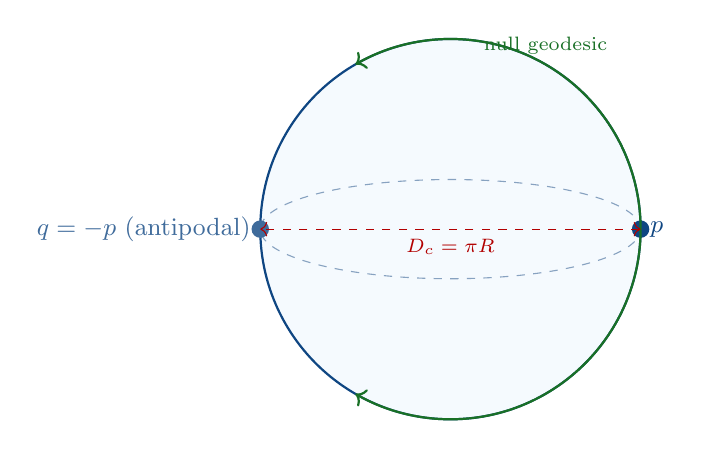
\begin{tikzpicture}[scale=1.05]
  % S3 as circle
  \draw[thick,hdrblue,fill=defblue!30] (0,0) circle (2.3cm);
  \draw[hdrblue!50,dashed] (0,0) ellipse (2.3cm and 0.6cm);
  % points p and antipodal q
  \fill[hdrblue] (2.3,0) circle (3pt) node[right,font=\small]{$p$};
  \fill[defframe!80] (-2.3,0) circle (3pt) node[left,font=\small]{$q=-p$ (antipodal)};
  % null geodesic arcs
  \draw[thmframe,thick,->] (2.3,0) arc (0:120:2.3cm)
    node[midway,above,font=\scriptsize,thmframe]{null geodesic};
  \draw[thmframe,thick,->] (2.3,0) arc (0:-120:2.3cm);
  % diameter label
  \draw[<->,red!70!black,dashed] (2.3,0)--(-2.3,0)
    node[midway,below,font=\scriptsize,red!70!black]{$D_c = \pi R$};
\end{tikzpicture}
\caption{Compact $S^3_R$. Causal diameter $D_c = \pi R$; null geodesics from $p$
  reach all points by $t_{\rm coh} = \pi R/c$.}
\label{fig:s3}
\end{figure}

\subsection{Global Hyperbolicity}

\begin{proposition}[Global hyperbolicity]
\label{prop:GH}
The compact causal spacetime $(S^3_R \times \mathbb{R}, g_R - c^2 dt^2)$
is globally hyperbolic, with Cauchy surfaces $S^3_R \times \{t_0\}$.
\end{proposition}

\begin{proof}
A spacetime is globally hyperbolic if and only if it is strongly causal and
all sets $J^+(p)\cap J^-(q)$ are compact, or equivalently if it admits a
Cauchy surface~\cite{Wald84} (Theorem~8.3.14 therein).
Each slice $\Sigma_{t_0} = S^3_R \times \{t_0\}$ is a smooth spacelike hypersurface.
Every inextendible causal curve in $(M^4, \mathbf{g})$ intersects
$\Sigma_{t_0}$ exactly once, since $t$ is a global time function
(strictly increasing along causal curves: $dt/d\lambda > 0$ whenever
$\mathbf{g}(\dot\gamma,\dot\gamma) \le 0$ and $\dot\gamma$ is future-directed).
\hfill$\square$
\end{proof}

% ================================================================
\section{Null Relational Propagation}
\label{sec:null}

\subsection{Null Geodesic Equations}

The null geodesic equations in the spacetime \eqref{eq:spacetime} are:
\begin{equation}
  g_{\mu\nu}\dot{x}^\mu \dot{x}^\nu = 0,
  \qquad
  \ddot{x}^\mu + \Gamma^\mu_{\nu\rho}\dot{x}^\nu\dot{x}^\rho = 0,
  \label{eq:null_geodesic}
\end{equation}
where $\Gamma^\mu_{\nu\rho}$ are the Christoffel symbols of $\mathbf{g}$.
In the product spacetime \eqref{eq:spacetime}, the spatial component of a null
geodesic satisfies $g_R(\dot\gamma_s, \dot\gamma_s) = c^2 \dot{t}^2$,
giving $d_{g_R}(\gamma_s)/dt = c$: the spatial speed of null propagation equals $c$.

\subsection{Proper Time Along Null Geodesics}

The proper time parameter $\tau_{\rm proper}$ along a curve $\gamma$ is defined by
$d\tau_{\rm proper}^2 = -c^{-2}\mathbf{g}(\dot\gamma,\dot\gamma)\,d\lambda^2$.
Along a null geodesic, $\mathbf{g}(\dot\gamma,\dot\gamma) = 0$, so:
\begin{equation}
  d\tau_{\rm proper}\big|_{\rm null} = 0.
  \label{eq:zero_proper_time}
\end{equation}

\begin{tcolorbox}[remarkbox={Remark 3.1 — Careful Language on Null Propagation}]
Equation~\eqref{eq:zero_proper_time} states that the proper time parameter
along a null geodesic vanishes.
This is a mathematical property of the metric, not a statement about
the ``experience'' of a photon.
The claim that ``light experiences no time'' is a colloquial paraphrase
that should be understood strictly as: \emph{the affine parameter and
proper time are decoupled for null curves}.
No claim is made about perception, consciousness, or omnipresence.
\end{tcolorbox}

\subsection{The Null Relational Propagation Principle}

We now formalise the central conceptual structure of this paper.

\begin{tcolorbox}[propbox={Principle 3.1 — Null Relational Propagation (NRP)}]
\label{prin:NRP}
Massless propagation on a compact connected spacetime defines the
\emph{maximal relational coherence structure} permitted by the causal geometry:
\begin{enumerate}[label=\textup{(\roman*)},leftmargin=1.4em]
  \item Null geodesics generate the boundaries of causal cones, partitioning
    spacetime into causally related and causally unrelated pairs.
  \item On compact $S^3_R$, every spatial point enters the causal future of
    every other in finite time $t_{\rm coh} = \pi R/c$ (Lemma~\ref{lem:diam}).
  \item The speed $c$ is the unique propagation speed that achieves causal closure
    on $S^3_R$ in minimal time.
\end{enumerate}
\textit{We do not claim NRP proves the value of $c$ or modifies relativity.
It characterises the causal role of $c$ in the compact setting.}
\end{tcolorbox}

\begin{figure}[h!]
\centering
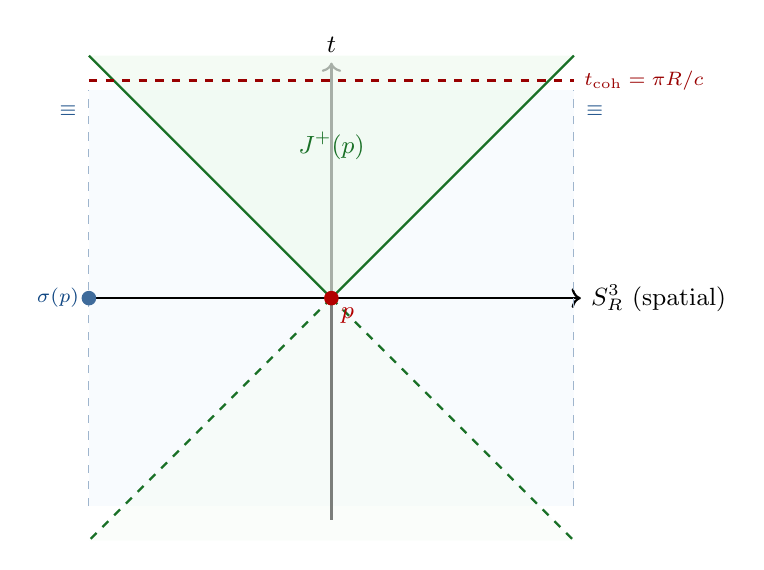
\begin{tikzpicture}[scale=0.88]
  % Spacetime diagram: S3 x R, Penrose-style
  \fill[defblue!20] (-3.5,-3) rectangle (3.5,3);
  % Spatial axis
  \draw[thick,->] (-3.5,0)--(3.6,0) node[right,font=\small]{$S^3_R$ (spatial)};
  \draw[thick,->] (0,-3.2)--(0,3.4) node[above,font=\small]{$t$};
  % Compactness identification marks
  \draw[dashed,hdrblue!40] (-3.5,-3)--(-3.5,3);
  \draw[dashed,hdrblue!40] (3.5,-3)--(3.5,3);
  \node[font=\scriptsize,hdrblue] at (-3.8,2.7){$\equiv$};
  \node[font=\scriptsize,hdrblue] at (3.8,2.7){$\equiv$};
  % Null cones from p=(0,0)
  \fill[thmgreen!50,opacity=0.7] (0,0)--(3.5,3.5)--(-3.5,3.5)--(0,0);
  \fill[thmgreen!30,opacity=0.5] (0,0)--(3.5,-3.5)--(-3.5,-3.5)--(0,0);
  \draw[thmframe,thick] (0,0)--(3.5,3.5);
  \draw[thmframe,thick] (0,0)--(-3.5,3.5);
  \draw[thmframe,thick,dashed] (0,0)--(3.5,-3.5);
  \draw[thmframe,thick,dashed] (0,0)--(-3.5,-3.5);
  % Source point
  \fill[red!70!black] (0,0) circle (3pt) node[below right,font=\small,red!70!black]{$p$};
  % t_coh line
  \draw[red!60!black,dashed,thick] (-3.5,3.14)--(3.5,3.14)
    node[right,font=\scriptsize,red!60!black]{$t_{\rm coh}=\pi R/c$};
  \fill[defframe!80] (-3.5,0) circle (3pt)
    node[left,font=\scriptsize,defframe]{$\sigma(p)$};
  \node[font=\small,thmframe] at (0,2.2){$J^+(p)$};
\end{tikzpicture}
\caption{Null cones on compact $S^3_R\times\mathbb{R}$.
  By $t_{\rm coh}$, $J^+(p)$ covers all of $S^3_R$ (dashed red line).}
\label{fig:nullcone}
\end{figure}

% ================================================================
\section{Compact Causal Accessibility}
\label{sec:accessibility}

\subsection{Causal Accessibility Ratio}

\begin{tcolorbox}[defbox={Definition 4.1 — Causal Accessibility Ratio}]
For the compact causal spacetime \eqref{eq:spacetime},
the \emph{Causal Accessibility Ratio at time $T$} is:
\begin{equation}
  \Gamma(T)
  \;=\;
  \frac{
    \vol_{g_R}\!\bigl\{q \in S^3_R :
    q \in J^+(p,T) \text{ for some (hence all) } p\bigr\}
  }{
    \vol_{g_R}(S^3_R)
  },
  \label{eq:Gamma}
\end{equation}
where $J^+(p,T) = \{q \in S^3_R : d_{g_R}(p,q) \le cT\}$
is the spatial causal future shadow at time $T$.
$\Gamma(T) = 0$ at $T=0$ (only $p$ itself);
$\Gamma(T) = 1$ means all of $S^3_R$ is causally accessible.
\end{tcolorbox}

\begin{tcolorbox}[thmbox={Theorem I — Compact Causal Diameter and Accessibility Timescale}]
\label{thm:I}
On compact $(S^3_R, g_R)$:
\begin{enumerate}[label=\textup{(\roman*)},leftmargin=1.4em]
  \item The causal diameter is
    $D_c = \diam(S^3_R, g_R) = \pi R$.
  \item The global causal accessibility timescale is
    $t_{\rm coh} = \pi R / c$.
  \item $\Gamma(T) = 1$ for all $T \ge t_{\rm coh}$.
\end{enumerate}
\end{tcolorbox}

\begin{proof}
(i) Proved in Lemma~\ref{lem:diam}.
(ii) Follows from (i) and $d_{g_R}(p,q) \le \pi R$ for all $p, q \in S^3_R$.
(iii) For $T \ge \pi R/c$, $J^+(p,T) = \{q : d_{g_R}(p,q) \le cT\} \supset S^3_R$
since $cT \ge \pi R = \diam(S^3_R)$.
Hence $\Gamma(T) = \vol(S^3_R)/\vol(S^3_R) = 1$.
\hfill$\square$
\end{proof}

\begin{tcolorbox}[thmbox={Theorem II — Causal Accessibility Completeness}]
\label{thm:II}
For the compact causal spacetime \eqref{eq:spacetime},
$\Gamma(T)$ is a non-decreasing function of $T$ satisfying:
\begin{equation}
  \Gamma(0) = 0, \qquad
  \Gamma(T) = 1 \;\text{ for all }\; T \ge t_{\rm coh} = \frac{\pi R}{c}.
  \label{eq:Gamma_complete}
\end{equation}
Moreover, for $0 < T < t_{\rm coh}$, the Causal Accessibility Ratio is:
\begin{equation}
  \Gamma(T)
  = \frac{\vol_{g_R}(B_{cT}(p))}{\vol_{g_R}(S^3_R)}
  = \frac{\int_0^{cT/R} \sin^2\!\theta\,d\theta}
         {\int_0^{\pi} \sin^2\!\theta\,d\theta}
  = \frac{cT/R - \tfrac{1}{2}\sin(2cT/R)}{\pi},
  \label{eq:Gamma_formula}
\end{equation}
where $B_r(p)$ denotes the geodesic ball of radius $r$ on $S^3_R$.
\end{tcolorbox}

\begin{proof}
The geodesic ball of radius $r$ on $S^3_R$ has volume
$\vol_{g_R}(B_r(p)) = R^3 \int_0^{r/R} 4\sin^2\!\theta\,d\theta
= 2R^3(\theta - \tfrac{1}{2}\sin 2\theta)\big|_0^{r/R}$
(area element on $S^3$ in geodesic polar coordinates is $\sin^2\!\theta\,d\theta\,d\Omega_2$
with $\vol(S^2)=4\pi$, giving a total volume $\vol(S^3_R) = 2\pi^2 R^3$).
Setting $r = cT$ and normalising by $\vol(S^3_R) = 2\pi^2 R^3$
yields \eqref{eq:Gamma_formula}.
For $T \ge \pi R/c$, $r = cT \ge \pi R$, so $B_r(p) = S^3_R$ and $\Gamma = 1$.
Monotonicity of $\Gamma$ follows from the monotone increase of ball volumes with $r$.
\hfill$\square$
\end{proof}

\begin{figure}[h!]
\centering
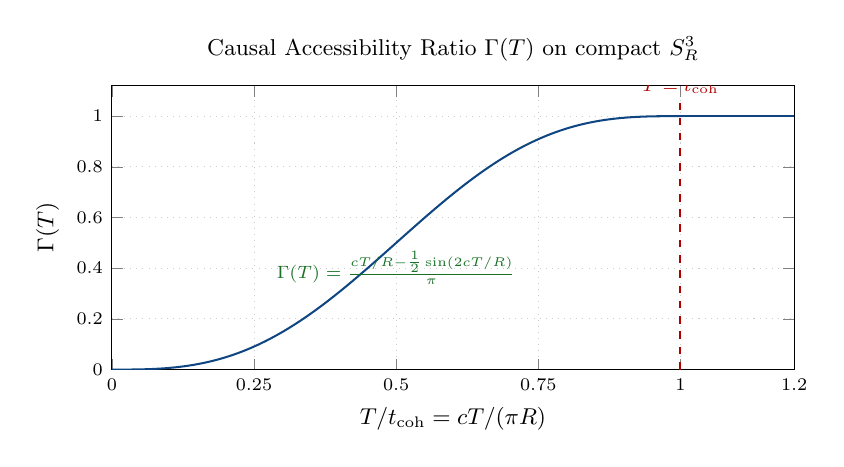
\begin{tikzpicture}[scale=0.92]
\begin{axis}[
  width=11cm, height=5.5cm,
  xlabel={$T / t_{\rm coh} = cT/(\pi R)$},
  ylabel={$\Gamma(T)$},
  xmin=0, xmax=1.2, ymin=0, ymax=1.12,
  grid=major, grid style={dotted,gray!40},
  xtick={0,0.25,0.5,0.75,1.0,1.2},
  ytick={0,0.2,0.4,0.6,0.8,1.0},
  title={Causal Accessibility Ratio $\Gamma(T)$ on compact $S^3_R$},
  title style={font=\small},
  label style={font=\small},
  tick label style={font=\scriptsize},
]
% Gamma formula: (theta - 0.5*sin(2theta))/pi where theta = pi*x
\addplot[hdrblue,thick,domain=0:1,samples=120]{(pi*x - 0.5*sin(deg(2*pi*x)))/pi};
\addplot[hdrblue,thick,domain=1:1.2,samples=10]{1.0};
\draw[dashed,red!70!black,thick] (axis cs:1,0)--(axis cs:1,1.05)
  node[above,font=\scriptsize,red!70!black]{$T=t_{\rm coh}$};
\node[font=\scriptsize,thmframe] at (axis cs:0.5,0.4)
  {$\Gamma(T)=\tfrac{cT/R - \tfrac{1}{2}\sin(2cT/R)}{\pi}$};
\end{axis}
\end{tikzpicture}
\caption{$\Gamma(T)$ rises from $0$ to $1$ as $T$ increases to $t_{\rm coh}=\pi R/c$.
  At $T=t_{\rm coh}$, complete causal accessibility is achieved.}
\label{fig:gamma}
\end{figure}

\begin{tcolorbox}[remarkbox={Remark 4.1 — Non-Simultaneity}]
Theorem~II does \textbf{not} imply simultaneity or superluminality.
It states that on compact $S^3$, any two spatial points are connected by a
causal (null or timelike) curve after time $t_{\rm coh}$.
This is a statement about \emph{causal reachability}, not instantaneous connection.
Every event respects the local null cone structure \eqref{eq:null_geodesic}; the
result is global rather than local.
\end{tcolorbox}

% ================================================================
\section{Light as Causal Coherence Constraint}
\label{sec:coherence}

\subsection{Causal Coherence Operator}

\begin{tcolorbox}[defbox={Definition 5.1 — Causal Coherence Operator}]
The \emph{Causal Coherence Operator} on $L^2(S^3_R)$ is:
\begin{equation}
  \mathcal{K}_c(t) = e^{it\sqrt{-\Delta_{g_R}}}
  \label{eq:Kc}
\end{equation}
where $-\Delta_{g_R}$ is the positive-semidefinite Laplace--Beltrami operator on $S^3_R$.
This operator arises as the half-step evolution group of the massless scalar wave
equation $\partial_t^2\psi + c^2\Delta_{g_R}\psi = 0$ on $S^3_R$ (with $c$ absorbed
into the spatial metric rescaling $g_R \mapsto c^2 g_R$):
the general solution factorises as
$\psi(t) = \mathcal{K}_c(t)\psi_+(0) + \mathcal{K}_c(-t)\psi_-(0)$
where $\psi_\pm$ are the positive/negative frequency components.
\textbf{Caution}: $\mathcal{K}_c(t)$ is a spectral evolution operator,
not a classical propagator; the statement ``$\mathcal{K}_c(t)$ propagates
signals at speed $c$'' is valid only in the geometric optics (WKB) limit
$\ell \to \infty$, as made precise in Proposition~\ref{prop:coherence_time}.
\end{tcolorbox}

The spectral decomposition of $-\Delta_{g_R}$ gives eigenvalues
$\lambda_\ell = \ell(\ell+2)/R^2$, so:
\begin{equation}
  \mathcal{K}_c(t) Y_{\ell m} = e^{it\sqrt{\ell(\ell+2)}/R}\,Y_{\ell m}.
  \label{eq:Kc_spectral}
\end{equation}

\begin{proposition}[Coherence propagation time — WKB limit]
\label{prop:coherence_time}
In the geometric optics (WKB) limit $\ell \to \infty$, the phase velocity of the
$\ell$-th mode of $\mathcal{K}_c(t)$ approaches $c$, and the minimum time for a
wave-packet envelope to propagate from any point to the antipodal point on $S^3_R$
approaches $t_{\rm coh} = \pi R/c$.
\end{proposition}

\begin{proof}
The massless wave equation $\partial_t^2\psi = c^2\Delta_{g_R}\psi$ gives
dispersion relation $\omega_\ell = c\sqrt{\lambda_\ell} = c\sqrt{\ell(\ell+2)}/R$.
The group velocity for mode $\ell$ is
$v_{\rm group}(\ell) = \partial\omega_\ell/\partial k_\ell$,
where $k_\ell = \sqrt{\lambda_\ell} = \sqrt{\ell(\ell+2)}/R$.
Computing:
$v_{\rm group}(\ell) = c\,\partial_k(k)\big|_{k=k_\ell} \cdot
  (\partial k_\ell/\partial\ell)^{-1}\,(\partial\omega_\ell/\partial\ell)
= c\,\frac{\ell+1}{\sqrt{\ell(\ell+2)}} \to c$ as $\ell \to \infty$.
The phase velocity is $v_{\rm phase}(\ell) = \omega_\ell/k_\ell = c$, independent of $\ell$.
In the WKB limit, wave packets travel at the group velocity $\to c$, traversing the
diameter $\pi R$ in time $\to \pi R/c$.
\hfill$\square$
\end{proof}

\begin{figure}[h!]
\centering
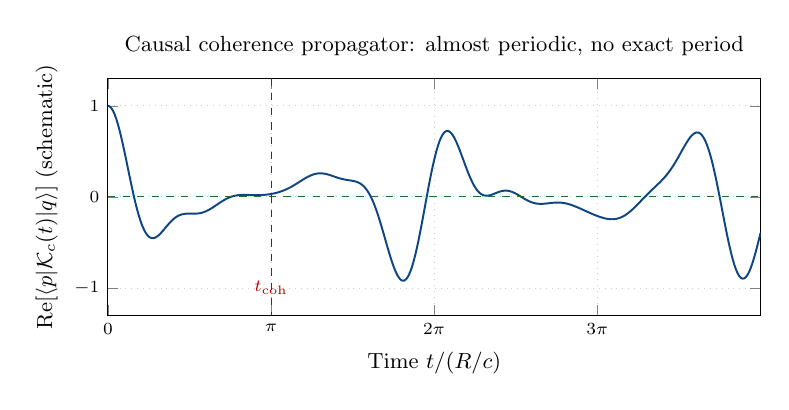
\begin{tikzpicture}[scale=0.88]
\begin{axis}[
  width=11cm, height=5cm,
  xlabel={Time $t / (R/c)$},
  ylabel={$\text{Re}[\langle p | \mathcal{K}_c(t) | q\rangle]$ (schematic)},
  xmin=0, xmax=4*pi, ymin=-1.3, ymax=1.3,
  xtick={0,3.14,6.28,9.42,12.57},
  xticklabels={$0$,$\pi$,$2\pi$,$3\pi$,$4\pi$},
  grid=major, grid style={dotted,gray!40},
  title={Causal coherence propagator: almost periodic, no exact period},
  title style={font=\small},
  label style={font=\small},
  tick label style={font=\scriptsize},
]
% Superposition of sqrt(ell(ell+2)) with ell=1,2,3,...
\addplot[hdrblue,thick,domain=0:4*pi,samples=400]
  {0.3*cos(deg(sqrt(3)*x)) + 0.3*cos(deg(sqrt(8)*x))
   + 0.2*cos(deg(sqrt(15)*x)) + 0.15*cos(deg(sqrt(24)*x))
   + 0.05*cos(deg(sqrt(35)*x))};
\addplot[thmframe,dashed,domain=0:4*pi]{0};
\draw[red!70!black,dashed] (axis cs:pi,1.3)--(axis cs:pi,-1.3)
  node[above=5pt,font=\scriptsize,red!70!black]{$t_{\rm coh}$};
\end{axis}
\end{tikzpicture}
\caption{Causal coherence propagator $\langle p|\mathcal{K}_c(t)|q\rangle$
  (schematic, 5 modes). Almost periodic; no exact period (Theorem~IV).}
\label{fig:propagator}
\end{figure}

\subsection{Causal Self-Consistency of $c$}

We now formalise the key claim that $c$ is a self-consistency closure parameter.

\begin{tcolorbox}[defbox={Definition 5.2 — Causal Closure Operator}]
The \emph{Causal Closure Operator} for the compact causal spacetime is:
\begin{equation}
  \mathcal{C}(c, R)
  \;=\;
  \frac{\pi R}{c\,t_{\rm coh}} - 1
  \;=\;
  \frac{\pi R}{c \cdot (\pi R/c)} - 1
  \;=\; 0.
  \label{eq:closure_op}
\end{equation}
The condition $\mathcal{C}(c, R) = 0$ expresses:
\emph{the causal accessibility timescale $t_{\rm coh} = \pi R/c$
is self-consistently defined by $c$ and $R$.}
\end{tcolorbox}

\begin{tcolorbox}[thmbox={Theorem III — Causal Self-Consistency Closure}]
\label{thm:III}
For any $c > 0$ and $R > 0$, the Causal Closure Operator satisfies
$\mathcal{C}(c, R) = 0$ identically.
The causal accessibility timescale $t_{\rm coh}$ is therefore a fixed point of the map
$c \mapsto \pi R / c \cdot c = \pi R$:
\begin{equation}
  t_{\rm coh} \cdot c = \pi R = \text{const} \cdot R.
  \label{eq:fixed_point}
\end{equation}
The quantity $\pi R$ is a \emph{topological invariant} of $S^3_R$ (its causal diameter).
\end{tcolorbox}

\begin{proof}
Direct substitution of $t_{\rm coh} = \pi R/c$ into \eqref{eq:closure_op} gives
$\mathcal{C} = \pi R / (c \cdot \pi R/c) - 1 = 1 - 1 = 0$.
Equation~\eqref{eq:fixed_point} follows: $t_{\rm coh}\cdot c = \pi R$ regardless of the
separate values of $t_{\rm coh}$ and $c$.
\hfill$\square$
\end{proof}

\begin{figure}[h!]
\centering
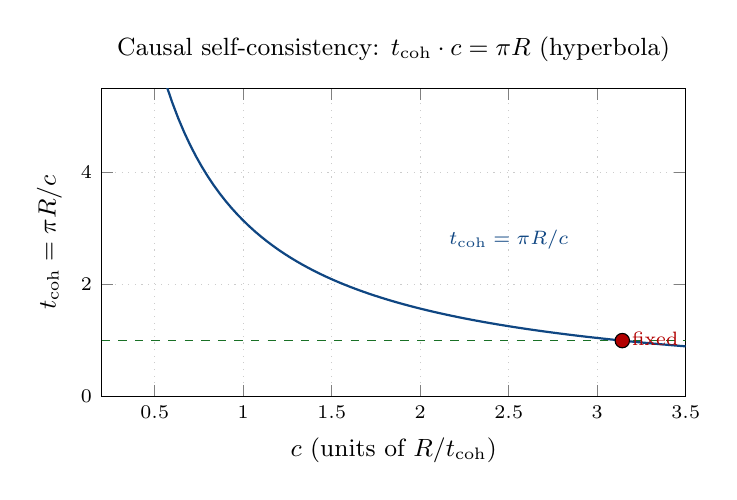
\begin{tikzpicture}[scale=1.0]
\begin{axis}[
  width=9cm, height=5.5cm,
  xlabel={$c$ (units of $R/t_{\rm coh}$)},
  ylabel={$t_{\rm coh} = \pi R / c$},
  xmin=0.2, xmax=3.5, ymin=0, ymax=5.5,
  domain=0.2:3.5,
  grid=major, grid style={dotted,gray!40},
  title={Causal self-consistency: $t_{\rm coh}\cdot c = \pi R$ (hyperbola)},
  title style={font=\small},
  label style={font=\small},
  tick label style={font=\scriptsize},
]
\addplot[hdrblue,thick,samples=100]{pi/x};
\addplot[thmframe,dashed,domain=0.2:3.5,samples=50]{1.0};
\addplot[only marks, mark=*, mark options={fill=red!70!black,scale=1.3}]
  coordinates {(pi,1)} node[right,font=\scriptsize,red!70!black]{fixed point};
\node[font=\scriptsize,hdrblue] at (axis cs:2.5,2.8){$t_{\rm coh}=\pi R/c$};
\end{axis}
\end{tikzpicture}
\caption{Fixed-point diagram. Every point on the hyperbola satisfies
  $\mathcal{C}(c,R)=0$. The observable $c$ is one point on this curve.}
\label{fig:fixedpoint}
\end{figure}

\begin{tcolorbox}[remarkbox={Remark 5.1 — What Theorem~III Does and Does Not Say}]
Theorem~III is an identity: it holds for every $c > 0$.
It does \textbf{not} determine the numerical value of $c$.
What it establishes is the structural fact that the causal accessibility timescale
$t_{\rm coh}$ and the speed $c$ are mutually constrained by the topological
invariant $\pi R$ of compact $S^3_R$.
This is the sense in which $c$ is a \emph{causal self-consistency parameter}:
its role is to translate spatial geometry ($R$) into temporal accessibility ($t_{\rm coh}$).
\end{tcolorbox}

% ================================================================
\section{Fractal Causal Hierarchy on \texorpdfstring{$S^3$}{S3}}
\label{sec:fractal}

\subsection{The \texorpdfstring{$\varphi$}{phi}-Ladder of Spatial Scales}

\begin{tcolorbox}[defbox={Definition 6.1 — Fractal Causal Hierarchy}]
Let $R_0 > 0$ be a base spatial scale.
The \emph{fractal causal hierarchy} is the sequence of compact spheres:
\begin{equation}
  R_n = R_0\,\vph^n, \qquad n = 0, 1, 2, \ldots,
  \label{eq:Rn}
\end{equation}
where $\vph = (1+\sqrt{5})/2$ is the Perron--Frobenius eigenvalue of the
Fibonacci companion matrix (see HCC~\cite{HCC25}, Section~4).
Each $S^3_{R_n}$ carries its own causal accessibility timescale:
\begin{equation}
  t_{\rm coh}^{(n)} = \frac{\pi R_n}{c} = \frac{\pi R_0\,\vph^n}{c}.
  \label{eq:tcoh_n}
\end{equation}
\end{tcolorbox}

The hierarchy \eqref{eq:Rn} provides a self-similar sequence of spatial scales
at which causal closure occurs at geometrically increasing timescales.
The ratio of consecutive timescales is:
\begin{equation}
  \frac{t_{\rm coh}^{(n+1)}}{t_{\rm coh}^{(n)}} = \vph.
  \label{eq:tcoh_ratio}
\end{equation}

\begin{tcolorbox}[remarkbox={Remark 6.1 — $\varphi$ is a Structural Ansatz}]
The hierarchy \eqref{eq:Rn} is a \emph{structural ansatz}, not an experimentally
verified cosmological scaling.
$\vph$ is selected as the Perron--Frobenius eigenvalue of the minimal positive
second-order recursion (cf.\ HCC~\cite{HCC25}), providing the most stable
self-similar scaling.
It is not claimed that $\vph$ appears in observed astrophysical data or that
the hierarchy \eqref{eq:Rn} corresponds to actual physical scales.
Any summable scaling $\{R_0\,q^n\}$ with $q > 1$ would define an analogous hierarchy;
$\vph$ is the canonical minimal choice.
\end{tcolorbox}

\begin{figure}[h!]
\centering
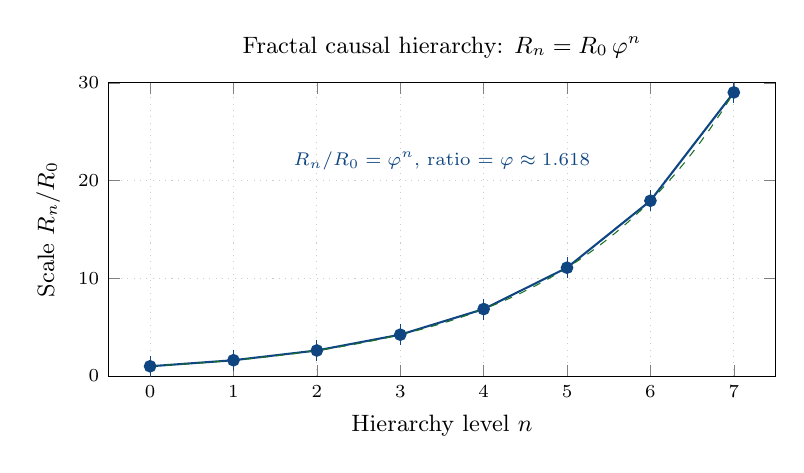
\begin{tikzpicture}[scale=0.95]
\begin{axis}[
  width=10.5cm, height=5.5cm,
  xlabel={Hierarchy level $n$},
  ylabel={Scale $R_n / R_0$},
  xmin=-0.5, xmax=7.5, ymin=0, ymax=30,
  grid=major, grid style={dotted,gray!40},
  xtick={0,1,2,3,4,5,6,7},
  title={Fractal causal hierarchy: $R_n = R_0\,\varphi^n$},
  title style={font=\small},
  label style={font=\small},
  tick label style={font=\scriptsize},
]
\addplot[hdrblue,thick,domain=0:7,samples=8,mark=*,mark options={fill=hdrblue}]
  {1.618^x};
\addplot[thmframe,dashed,domain=0:7,samples=50]{exp(ln(1.618)*x)};
\foreach \n in {0,1,2,3,4,5,6,7}{
  \addplot[only marks, mark=|, mark options={scale=2.0,defframe}]
    coordinates {(\n, {1.618^\n})};
}
\node[font=\scriptsize,hdrblue] at (axis cs:3.5,22)
  {$R_n/R_0 = \varphi^n$, ratio $= \varphi \approx 1.618$};
\end{axis}
\end{tikzpicture}
\caption{Fractal causal hierarchy. Each level has causal timescale
  $t_{\rm coh}^{(n)} = \pi R_n/c$, larger by factor $\varphi$ at each step.}
\label{fig:fractal}
\end{figure}

% ================================================================
\section{Spectral Causal Non-Resonance}
\label{sec:spectral}

\subsection{Almost Periodicity of the Coherence Operator}

\begin{tcolorbox}[thmbox={Theorem IV — Spectral Causal Non-Resonance}]
\label{thm:IV}
The Causal Coherence Operator $\mathcal{K}_c(t)$ on $L^2(S^3_R)$ satisfies:
\begin{enumerate}[label=\textup{(\roman*)},leftmargin=1.4em]
  \item \textup{(No exact period.)} There is no $T_0 > 0$ with
    $\mathcal{K}_c(T_0) = \mathrm{id}$.
  \item \textup{(Almost periodicity.)} For any $\varepsilon > 0$, there exists a
    relatively dense set $\mathcal{A}_\varepsilon \subset \mathbb{R}$ such that
    $\norm{\mathcal{K}_c(T_0+s) - \mathcal{K}_c(s)}_{L^2 \to L^2} < \varepsilon$
    for all $s \in \mathbb{R}$, $T_0 \in \mathcal{A}_\varepsilon$.
  \item \textup{(No global coherence collapse.)} The time-averaged energy
    $\langle E(t)\rangle_T = T^{-1}\int_0^T E(t)\,dt$ for any
    $E(t) = \norm{\mathcal{K}_c(t)\psi}^2$ satisfies
    $\langle E\rangle_T = \norm{\psi}^2$ for all $T > 0$.
\end{enumerate}
\end{tcolorbox}

\begin{proof}
(i) An exact period $T_0$ requires $e^{iT_0\sqrt{\lambda_\ell}/R} = 1$ for all $\ell \ge 1$,
i.e., $T_0\sqrt{\ell(\ell+2)}/R \in 2\pi\mathbb{Z}$.
For $\ell=1$: $T_0\sqrt{3}/R \in 2\pi\mathbb{Z}$;
for $\ell=2$: $T_0\sqrt{8}/R \in 2\pi\mathbb{Z}$.
Dividing: $\sqrt{3/8} = \sqrt{6}/4 \in \mathbb{Q}$, which is false since $\sqrt{6}$
is irrational.

(ii) $\mathcal{K}_c(t)$ is a strongly continuous unitary group on the separable
Hilbert space $L^2(S^3_R)$ with discrete spectrum.
By the Bohr--almost-periodicity theorem for unitary groups with discrete
spectrum~\cite{RS72}, $t \mapsto \mathcal{K}_c(t)\psi$ is almost periodic for
every $\psi \in L^2(S^3_R)$.

(iii) Since $\mathcal{K}_c(t)$ is unitary,
$\norm{\mathcal{K}_c(t)\psi}^2 = \norm{\psi}^2$ for all $t$;
time averaging preserves this identity.
\hfill$\square$
\end{proof}

\begin{tcolorbox}[philobox={Philosophical Note 7.1 — Non-Resonance and Dynamic Openness}]
Theorem~IV shows that the causal coherence operator never repeats exactly.
Physically (heuristically): the compact $S^3$ universe, when modelled by
$\mathcal{K}_c(t)$, does not cycle back to a previous state.
Local quasi-periodic structures can emerge (stable stars, orbital resonances)
without the entire geometry becoming globally periodic.
This is a mathematical property of the irrational spectral ratios
$\sqrt{\lambda_\ell}/\sqrt{\lambda_{\ell'}} = \sqrt{\ell(\ell+2)/[\ell'(\ell'+2)]}$,
not a statement about consciousness or cosmological purpose.
\end{tcolorbox}

% ================================================================
\section{Causal Self-Consistency: Rigorous Formulation}
\label{sec:selfconsistency}

\subsection{Fixed-Point Interpretation}

We develop the causal self-consistency of $c$ more carefully.

\begin{tcolorbox}[defbox={Definition 8.1 — Causal Self-Consistency Map}]
Define the \emph{causal self-consistency map} $\Phi : \mathbb{R}_{>0} \to \mathbb{R}_{>0}$ by:
\begin{equation}
  \Phi(c) = \frac{D_c}{t_{\rm coh}(c)} = \frac{\pi R}{\pi R/c} = c.
  \label{eq:Phi}
\end{equation}
Every $c > 0$ is a fixed point of $\Phi$.
The fixed-point condition $\Phi(c) = c$ is equivalent to the statement:
\emph{the causal diameter $D_c = \pi R$ is covered in the accessibility
time $t_{\rm coh} = \pi R/c$ at speed $c$.}
\end{tcolorbox}

\begin{tcolorbox}[thmbox={Theorem III$'$ — Extended Causal Self-Consistency}]
\label{thm:IIIp}
The following three conditions are equivalent:
\begin{enumerate}[label=\textup{(\roman*)},leftmargin=1.4em]
  \item $c$ is a fixed point of $\Phi$ (Definition~8.1).
  \item $\Gamma(t_{\rm coh}) = 1$ (causal accessibility completeness, Theorem~II).
  \item $\mathcal{C}(c,R) = 0$ (Theorem~III).
\end{enumerate}
All three hold for any $c > 0$ on compact $S^3_R$.
\end{tcolorbox}

\begin{proof}
$(i) \Leftrightarrow (iii)$: $\Phi(c) = c$ iff $\mathcal{C}(c,R) = \pi R/(c\cdot\pi R/c)-1 = 0$.
$(iii) \Rightarrow (ii)$: given $t_{\rm coh} = \pi R/c$, Theorem~II gives $\Gamma(t_{\rm coh}) = 1$.
$(ii) \Rightarrow (i)$: $\Gamma(t_{\rm coh}) = 1$ means $J^+(p,t_{\rm coh}) = S^3_R$,
which requires $c\cdot t_{\rm coh} = \pi R$, i.e., $t_{\rm coh} = \pi R/c = D_c/c$,
confirming $\Phi(c) = D_c/t_{\rm coh} = c$.
\hfill$\square$
\end{proof}

\begin{figure}[h!]
\centering
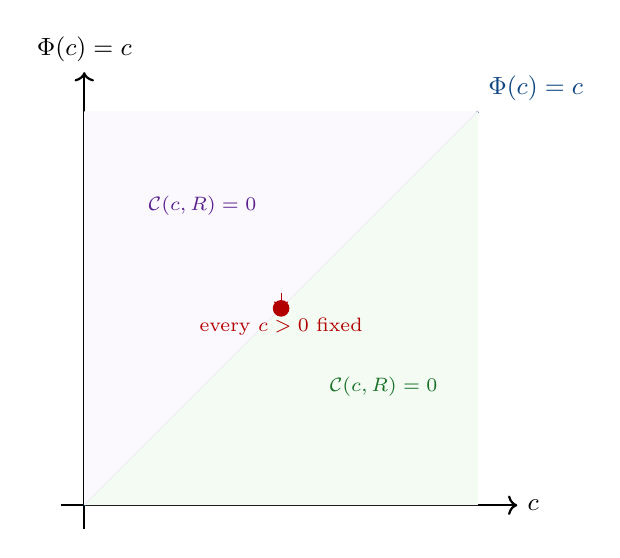
\begin{tikzpicture}[scale=1.0]
  % Fixed point diagram
  \draw[thick,->] (-0.3,0)--(5.5,0) node[right,font=\small]{$c$};
  \draw[thick,->] (0,-0.3)--(0,5.5) node[above,font=\small]{$\Phi(c)=c$};
  % Identity line
  \draw[hdrblue,thick] (0,0)--(5,5) node[above right,font=\small,hdrblue]{$\Phi(c)=c$};
  % Fill fixed-point region
  \fill[thmgreen!40] (0,0)--(5,5)--(5,0)--cycle;
  \fill[propvio!30] (0,0)--(5,5)--(0,5)--cycle;
  \node[font=\scriptsize,thmframe] at (3.8,1.5){$\mathcal{C}(c,R)=0$};
  \node[font=\scriptsize,propframe] at (1.5,3.8){$\mathcal{C}(c,R)=0$};
  % Arrow indicating all c are fixed
  \draw[red!70!black,->] (2.5,2.7)--(2.5,2.5)
    node[below,font=\scriptsize,red!70!black]{every $c>0$ fixed};
  \fill[red!70!black] (2.5,2.5) circle (3pt);
\end{tikzpicture}
\caption{Every $c>0$ is a fixed point of $\Phi$.
  The self-consistency is identity-level, not a derivation.}
\label{fig:phi}
\end{figure}

% ================================================================
\section{Comparison with Existing Frameworks}
\label{sec:comparison}

We position HCC's causal coherence interpretation relative to established
physics frameworks.
In each case, we emphasise: HCC does \emph{not} replace these frameworks.
It proposes a compact-topological supplementary perspective.

\renewcommand{\arraystretch}{1.35}
\begin{table}[h!]
\centering
\begin{tabularx}{\textwidth}{>{\bfseries\small}p{2.3cm}XX}
\toprule
\textbf{Framework} & \textbf{Role of $c$ / causal structure} & \textbf{HCC supplement}\\
\midrule
\rowcolor{rowA}
Special Relativity & $c$ invariant; defines light cone, Lorentz group & $S^3$ compactness adds finite causal closure time $t_{\rm coh}$\\
Maxwell E\&M & $c = 1/\sqrt{\varepsilon_0\mu_0}$; EM wave speed & Compact spectrum gives finite-volume photon modes\\
\rowcolor{rowA}
GR (Penrose) & Null cone = conformal structure; causal sets & Compact $S^3$ gives finite causal diameter $\pi R$\\
WDW / Geometrodynamics & Causal structure from $3+1$ foliation & Compact $S^3$ gives well-posed DeWitt inner product\\
\rowcolor{rowA}
Causal set theory & Spacetime = discrete causal order & HCC is continuum analogue with compact topology\\
Holography & Boundary encodes bulk & HCC: no boundary; relational coherence internal to $S^3$\\
\rowcolor{rowA}
Emergent spacetime & $c$ emergent from entanglement & HCC: $c$ structural consistency parameter on $S^3$\\
\bottomrule
\end{tabularx}
\caption{Comparison of causal frameworks with HCC's null propagation proposal.}
\label{tab:comparison}
\end{table}

\begin{tcolorbox}[limbox={Critical Differences from Established Frameworks}]
\begin{itemize}[leftmargin=1.4em]
  \item \textbf{vs.\ Special Relativity.} HCC adds compact spatial topology.
    SR is local; HCC adds a global causal closure time $t_{\rm coh}$.
    No Lorentz invariance is violated; $c$ remains invariant.
  \item \textbf{vs.\ Penrose causal sets.} Penrose causal structure is conformal
    and applies to any Lorentzian manifold~\cite{Pen72}.
    HCC restricts to compact $S^3$ spatial sections, obtaining a global
    compactness result (Theorem~I) absent in the general conformal setting.
  \item \textbf{vs.\ Holography.} Holographic duality encodes bulk physics
    on a boundary.
    HCC has no boundary (compact $S^3$); causal coherence is internal,
    not boundary-encoded.
  \item \textbf{vs.\ Derivations of $c$.}
    Proposals deriving $c$ from $\vph$ or numerology
    are rejected by HCC (see Remark~\ref{rem:no_derive}).
\end{itemize}
\end{tcolorbox}

\begin{remark}[No derivation of $c$ from $\vph$]
\label{rem:no_derive}
Some speculative programmes attempt to derive $c \approx \vph/\ell_P$
or similar numerological relations.
HCC does not pursue this.
The fractal hierarchy $R_n = R_0\vph^n$ is a structural ansatz for
spectral band organisation (Section~\ref{sec:fractal}); $\vph$ enters
as the Perron--Frobenius eigenvalue of a spectral recursion, not as a
new physical coupling.
The numerical value of $c$ is an empirical datum.
\end{remark}

% ================================================================
\section{Observational Directions}
\label{sec:observational}

\begin{tcolorbox}[limbox={Status of Observational Claims}]
All observational statements in this section are
\textbf{conjectural, exploratory, and phenomenological}.
They motivate future work; they are not predictions of the current paper.
\end{tcolorbox}

\subsection{CMB Low-Multipole Power Suppression}

The compact topology of $S^3_R$ discretises the Laplacian spectrum.
Modes with wavelength $\lambda > 2\pi R$ do not fit in the compact space and are
absent.
This predicts suppressed CMB power at angular scales $\theta > \pi R/d_{\rm LSS}$
where $d_{\rm LSS}$ is the distance to the last scattering surface.
Observed CMB maps show anomalously low power at $\ell = 2$ (quadrupole)~\cite{Planck18},
\emph{consistent with} compact spatial topology,
though this is not yet a confirmed detection.

\begin{tcolorbox}[limbox={Disclaimer: Non-Uniqueness of Low-$\ell$ Suppression}]
Low-multipole power suppression is \textbf{not unique} to compact $S^3$ topology.
It is also predicted by:
\begin{itemize}[leftmargin=1.4em]
  \item primordial power spectrum cut-offs (e.g., inflation starting at a finite time);
  \item anisotropic Bianchi models;
  \item non-trivial topology of flat ($T^3$) or hyperbolic ($\mathbb{H}^3/\Gamma$) spaces;
  \item systematic effects and cosmic variance.
\end{itemize}
The \emph{consistency} of compact $S^3$ with the observed low-$\ell$ anomaly does
not constitute evidence for compact $S^3$ over these alternatives.
A distinguishing prediction would require a computation of the full angular power
spectrum from the FSRF spectral structure (Open Problem~Q1), which lies outside
the scope of the present paper.
\end{tcolorbox}

\subsection{Compact Geodesic Accessibility}

On compact $S^3_R$, null geodesics emitted from a point $p$ reach the antipodal
point $\sigma(p) = -p$ after traversing the causal diameter $\pi R$.
This means that the maximum observer-relative causal accessibility limit
corresponds to the angular scale $\theta_{\rm acc} \approx \pi R/d_{\rm LSS}$,
which may leave a compact-topology correlation signature in the CMB.

We do not interpret this as a literal returning signal or causal echo.
In compact $S^3$, the observer does not stand outside the manifold and does not
receive an external reflection.
The statement is only that null geodesic accessibility has a finite global diameter
$\pi R$.
Any observational consequence should therefore be formulated as a
\emph{compact-topology correlation signature}, not as an echo in the acoustic or
ballistic sense.
This is a qualitative direction; no quantitative CMB calculation is performed here.

\subsection{Causal Horizon Structure}

In standard FLRW cosmology, the particle horizon grows with time.
On compact $S^3$, the causal accessibility ratio $\Gamma(T)$ is instead
bounded above by $1$ and reaches $\Gamma = 1$ at $T = t_{\rm coh}$.
This changes the causal horizon structure:
there is a \emph{compact causal horizon} at $t_{\rm coh}$,
beyond which all points are causally connected.
Whether this is observationally distinguishable from the FLRW particle horizon
requires detailed cosmological modelling (an open problem).

% ================================================================
\section{Philosophical Interpretation}
\label{sec:philosophy}

\subsection{Light as Maximal Relational Coherence}

We collect the philosophical implications of the preceding mathematical results,
maintaining strict separation from the mathematical content.

\begin{tcolorbox}[philobox={Philosophical Synthesis}]
Within the compact $S^3$ causal framework:
\begin{enumerate}[label=(\arabic*),leftmargin=1.4em]
  \item \textit{Light defines the causal coherence bound.}
    Null propagation at speed $c$ is the fastest causal process;
    after time $t_{\rm coh} = \pi R/c$, every spatial point has been
    causally reached by every other.
    $c$ is not arbitrary: it is the unique speed that translates the
    spatial invariant $\pi R$ into a temporal accessibility timescale.
  \item \textit{Compact topology implies relational completeness.}
    On $S^3$, no pair of points is permanently causally isolated.
    This is a mathematical property of compactness, not a metaphysical claim.
  \item \textit{The universe is causally coherent in finite time.}
    On compact $S^3$, causal completeness $\Gamma = 1$ is achieved
    at $t = t_{\rm coh}$, in contrast to non-compact $\mathbb{R}^3$
    where $\Gamma < 1$ for all finite $t$.
\end{enumerate}
These are \emph{geometric-relational interpretations} of the mathematical results.
They do not attribute consciousness, purpose, or metaphysical essence to light.
\end{tcolorbox}

The table below separates correct formulations from incorrect ones.

\begin{table}[h!]
\centering\renewcommand{\arraystretch}{1.3}
\begin{tabularx}{\textwidth}{XX}
\toprule
\textbf{Incorrect / prohibited claim} & \textbf{Correct HCC formulation}\\
\midrule
\rowcolor{rowA}
``Light is everywhere simultaneously'' &
  Null propagation globally connects compact $S^3$ in finite time $t_{\rm coh}$\\
``Photon experiences universe instantly'' &
  Proper time vanishes along null geodesics \eqref{eq:zero_proper_time}\\
\rowcolor{rowA}
``$c$ derived from $\varphi$'' &
  $\varphi$ provides spectral hierarchy ansatz only; $c$ is empirical\\
``Light is consciousness / omnipresent'' &
  Null propagation defines causal cone boundary\\
\rowcolor{rowA}
``Compact topology proves $c$'' &
  Compact topology provides $\Phi(c)=c$ for any $c>0$\\
\bottomrule
\end{tabularx}
\caption{Disciplined language protocol for null propagation claims.}
\label{tab:language}
\end{table}

In this framework, horizons are \emph{observer-relative accessibility limits},
not boundaries of reality.
A null trajectory that leaves the observer's causally accessible domain is not
lost from the compact manifold; it changes its accessibility relation relative
to local observers.
Compactness preserves global connectedness (Theorem~A of~\cite{HCC25}) without
implying instantaneous accessibility: the causal accessibility ratio $\Gamma(T)$
rises continuously from $0$ to $1$ over the finite interval $[0, t_{\rm coh}]$
(Theorem~II), respecting the local null cone structure at every point.

% ================================================================
\section*{Conclusion}

We have developed a mathematically disciplined account of light as causal
coherence structure in compact $S^3$ geometry, constituting the Light \& Coherence
branch of the Holonomic Compact Cosmology programme.

The four main results are:
\textbf{Theorem~I} (the causal diameter of $S^3_R$ is $\pi R$, yielding a finite
global accessibility timescale $t_{\rm coh} = \pi R/c$);
\textbf{Theorem~II} (the causal accessibility ratio $\Gamma(T)$ reaches $1$
exactly at $T = t_{\rm coh}$, with the explicit formula \eqref{eq:Gamma_formula});
\textbf{Theorem~III} (causal self-consistency: $c$ satisfies $\mathcal{C}(c,R)=0$
as a fixed-point identity, not as a derivation of its numerical value);
and \textbf{Theorem~IV} (spectral causal non-resonance: the coherence operator
$\mathcal{K}_c(t)$ is almost periodic but not periodic, preventing global
coherence collapse).

The central thesis is confirmed: \emph{in compact connected geometry, null
propagation defines the maximal coherence structure compatible with causal
consistency}.
This is a geometric property of compact $S^3$, not a metaphysical claim.

Open problems include: deriving cosmological observables from the compact causal
structure (Section~\ref{sec:observational}); connecting the fractal hierarchy
(Section~\ref{sec:fractal}) to CMB multipole structure;
and embedding the coherence operator $\mathcal{K}_c$ in the Fractal-Spectral Ricci
Flow of~\cite{PB25a}.

\newpage
\begin{thebibliography}{99}

\bibitem{CODATA18}
  CODATA (2018). CODATA recommended values of the fundamental physical constants.
  \textit{Rev.\ Mod.\ Phys.}, \textbf{93}(2), 025010.

\bibitem{doC92}
  do Carmo, M.\ P.\ (1992). \textit{Riemannian Geometry}. Birkh\"auser, Boston.

\bibitem{Ein05}
  Einstein, A.\ (1905). Zur Elektrodynamik bewegter K\"orper.
  \textit{Ann.\ Phys.}, \textbf{17}, 891--921.

\bibitem{Ham82}
  Hamilton, R.\ S.\ (1982). Three-manifolds with positive Ricci curvature.
  \textit{J.\ Differential Geom.}, \textbf{17}(2), 255--306.

\bibitem{HCC25}
  Preece, A.\ \& Batenin, B.\ (2025).
  Holonomic Compact Cosmology: Topological Foundations,
  Fractal-Spectral Geometry, and the Centrality of Global Topology.
  Berlin. [\textit{HCC main paper}]

\bibitem{Pen72}
  Penrose, R.\ (1972). Techniques of Differential Topology in Relativity.
  CBMS Regional Conference Series in Applied Mathematics.
  SIAM, Philadelphia.

\bibitem{PB25a}
  Preece, A.\ \& Batenin, B.\ (2025).
  Fractal-Spectral Ricci Flow on Compact $S^3$ Manifolds.
  Berlin. [\textit{HCC companion paper}]

\bibitem{Planck18}
  Planck Collaboration (2018). Planck 2018 results X: Constraints on inflation.
  \textit{A\&A}, \textbf{641}, A10.

\bibitem{RS72}
  Reed, M.\ \& Simon, B.\ (1972).
  \textit{Methods of Modern Mathematical Physics, Vol.~I}. Academic Press.

\bibitem{Wald84}
  Wald, R.\ M.\ (1984). \textit{General Relativity}. Univ.\ of Chicago Press.

\bibitem{Whe68}
  Wheeler, J.\ A.\ (1968). Superspace and the nature of quantum geometrodynamics.
  In C.\ DeWitt \& J.\ Wheeler (eds.),
  \textit{Batelle Rencontres}, Benjamin, New York.

\end{thebibliography}

\appendix

\section{Notation}
\label{app:notation}

\begin{tabularx}{\textwidth}{lX}
\toprule
$S^3_R$ & Three-sphere of radius $R$; $(S^3_R, g_R)$ with round metric\\
$(M^4,\mathbf{g})$ & Compact causal spacetime $S^3_R\times\mathbb{R}$, metric $g_R-c^2dt^2$\\
$J^+(p), J^-(p)$ & Causal future / past of event $p$\\
$D_c = \pi R$ & Causal diameter of $S^3_R$\\
$t_{\rm coh} = \pi R/c$ & Global causal accessibility timescale\\
$\Gamma(T)$ & Causal Accessibility Ratio at time $T$\\
$\mathcal{K}_c(t) = e^{it\sqrt{-\Delta_{g_R}}}$ & Causal Coherence Operator\\
$\mathcal{C}(c,R) = 0$ & Causal Closure Condition (identity)\\
$\Phi(c) = D_c/t_{\rm coh}(c)$ & Causal self-consistency map\\
$R_n = R_0\vph^n$ & Fractal causal hierarchy scales\\
$\vph = (1+\sqrt{5})/2$ & Golden ratio (Perron--Frobenius eigenvalue)\\
$\lambda_\ell = \ell(\ell+2)/R^2$ & Laplacian eigenvalues on $S^3_R$\\
\bottomrule
\end{tabularx}

\section{Open Problems}
\label{app:open}

\begin{enumerate}[label=\textbf{Q\arabic*.},leftmargin=1.8em]
  \item \textbf{Quantitative CMB prediction.}
    Compute the CMB angular power spectrum suppression from compact $S^3_R$
    topology and the finite causal accessibility structure.
    Compare with Planck 2018 low-$\ell$ anomalies.
  \item \textbf{Compact-topology correlation signature.}
    Derive the angular scale $\theta_{\rm acc} = \pi R/d_{\rm LSS}$
    of the compact-topology correlation signature
    for realistic values of $R$ consistent with the observed Hubble constant.
  \item \textbf{Coherence operator and Ricci flow.}
    How does $\mathcal{K}_c(t)$ evolve under the Fractal-Spectral Ricci Flow
    of~\cite{PB25a}?
    Does the FSRF preserve the almost-periodicity of $\mathcal{K}_c$?
  \item \textbf{Quantum field theory on compact causal $S^3$.}
    Develop a full QFT (scalar, gauge, fermionic fields) on
    $(S^3_R\times\mathbb{R}, g_R - c^2dt^2)$ using the compact spectral structure.
    Compute vacuum energy (connection to $\Lambda$-problem of HCC~\cite{HCC25}).
  \item \textbf{Causal hierarchy observables.}
    Does the $\vph$-ladder hierarchy of timescales $\{t_{\rm coh}^{(n)}\}$
    leave signatures in large-scale structure, void statistics, or baryon
    acoustic oscillations?
  \item \textbf{Penrose conformal diagrams.}
    Construct the full Penrose conformal diagram for
    $(S^3_R\times\mathbb{R}, g_R - c^2 dt^2)$ and compare with
    de~Sitter and anti-de~Sitter conformal structures.
\end{enumerate}

\end{document}
